\subsection{Spiral Image Transformer}

    As explained in the previous section (see Section \ref{sec:IntroSpiralModel}), the spiral model is a transformer-based model that employs a spiral architecture to process input data. 

    \subsubsection{Spiral}

    To convert the 3-dimensional data (color channels, image height, image width) into a spiral form, the data must be unrolled into one dimension, resulting in an output format of (color channels, spiral length). Consequently, the data width and the height dimensions must be squeezed into a single dimension. This new form can then be utilized similarly to the data in the Column Image Transformer. As the data is flattened into a single dimension, it allows for an easy addition of positional embedding. It is the same process as in the Column Image Transformer see \autoref{sec:CIT_PositionalEmbedding}.

    \subsubsection{Spiral generation}
    \label{sec:spiral_generation}
    The conversion of data into a spiral form needs to be highly efficient because the code block will execute for every image (batch) in the dataset. Therefore, a simple nested for loop is insufficient. In this example, fancy indexing is used to convert the data into a spiral form. Thus, the data tensor is indexed with a two-dimensional tensor containing the indices of the spiral form.

    At the start of the model training script, one indexing spiral is created to be used for all images in the dataset. The following code block illustrates the creation of the spiral index tensor.

\begin{figure}[H]
\centering
\begin{lstlisting}[language=Python]
def create_spiral(n): # n = width and height
    
    matrix = [[0] * n for _ in range(n)] # Initialize n x n matrix

    x, y = 0, 0
    # Direction vectors (right, down, left, up)
    dx = [0, 1, 0, -1]
    dy = [1, 0, -1, 0]
    direction = 0

    for i in range(n * n - 1, -1, -1):  # Start (35 for 6x6)
        matrix[x][y] = i
        nx = x + dx[direction]
        ny = y + dy[direction]

        # Change direction if the next position: out of bounds or filled
        if nx<0 or nx>=n or ny<0 or ny>=n or matrix[nx][ny]!=0:
            direction = (direction + 1) % 4  # Change direction
            nx = x + dx[direction]
            ny = y + dy[direction]

        x, y = nx, ny
    
    return torch.tensor(matrix)
\end{lstlisting}
\caption{Python function to create a spiral index tensor}
\label{fig:spiral_matrix}
\end{figure}

    The code above generates a square matrix of size n by n, then fills it with numbers in a spiral pattern, starting from the outer edge and spiraling inwards clockwise. Each cell of the matrix is assigned a unique number, beginning from the highest value in the top-left corner and decreasing by one with each step along the spiral path until reaching zero at the center or the end of the spiral. The spiral formation is achieved by moving right, then down, then left, then up, and repeating this sequence, adjusting direction whenever the next step would go out of bounds or into a cell that's already been filled.


    \subsection{Fancy Indexing into the Spiral form}

    The spiral index tensor is then used to index the data tensor, effectively converting it into a spiral form. The following image illustrates the process of converting a 7x7 image.
    
    
    \begin{figure}[H]
    \centering
    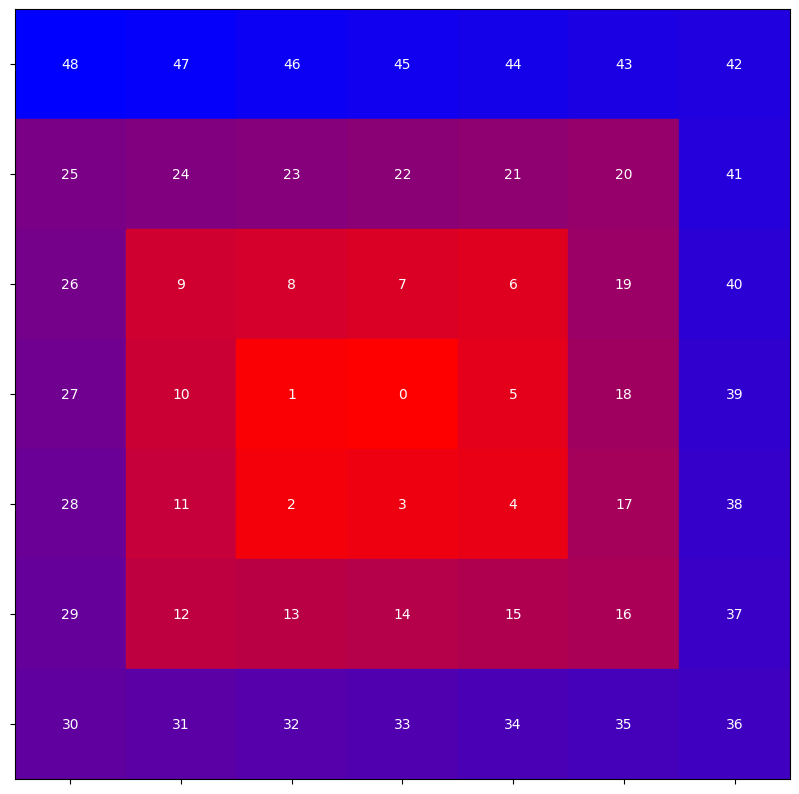
\includegraphics[width=0.6\textwidth]{../code/dataAnalysis/plots/exampleImgs/spiralShowcase1.png}
    \caption{Image representation}
    \label{fig:spiral_indexing_1}        
    \end{figure}

    \begin{figure}[H]
    \centering
    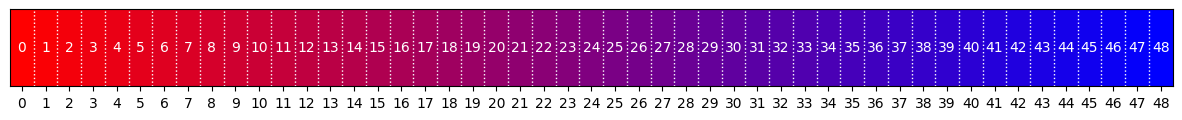
\includegraphics[width=1\textwidth]{../code/dataAnalysis/plots/exampleImgs/spiralShowcase0.png}
    \caption{7x7 Image flattened into a spiral form} 
    \label{fig:spiral_indexing_0}        
    \end{figure}

    As you can see in \autoref{fig:spiral_indexing_1}, the pixels of the image are labeled with their respective indices 0, \dots, 43. The image is then unrolled into a single dimension, as shown in \autoref{fig:spiral_indexing_0}. The centering pixel is the first element of the spiral, and the spiral continues counterclockwise from there. In the model script, the dimensions for width and height typically exceed 7, yet the underlying process remains unchanged.

\begin{figure}[H]
\centering
\begin{lstlisting}[language=Python]
  spiral_indices = torch.tensor(create_spiral(IMAGE_SIZE))

  # [...]
  # Batch_size, Color_channels, Height, Width
  B, C, H, W = data.shape

  spiral_data = torch.zeros_like(data.view(B, C, -1))

  spiral_data[:,:,spiral_indices.flatten()] = data.view(B, C, -1)

  # [...]
\end{lstlisting}
\caption{Fancy indexing to convert data into a spiral form}
\label{fig:spiral_indexing_code}
\end{figure}


